\documentclass[11pt,a4paper]{article}
\textheight245mm
\textwidth170mm
\hoffset-21mm
\voffset-15mm
\parindent0pt
\usepackage[utf8]{inputenc}
\usepackage{dsfont}
\usepackage{graphicx}
\usepackage{caption}
\usepackage{fancyhdr}
\usepackage{amsmath,amsfonts,amssymb}
\usepackage[french]{babel}
\usepackage[maxalphanames=99, maxnames=99, backend=bibtex, style=alphabetic, sorting=ynt]{biblatex}
\addbibresource{rapport.bib}
\usepackage[hidelinks]{hyperref} 
\hypersetup{
  colorlinks   = true,    % Colours links instead of ugly boxes
  urlcolor     = blue,    % Colour for external hyperlinks
  linkcolor    = black,    % Colour of internal links
  citecolor    = black      % Colour of citations
}
\usepackage{/home/hazdard/Documents/Tex/zephyr}
\pagestyle{fancy}

\usepackage{array,multirow,makecell}
\setcellgapes{4pt}
\makegapedcells
\newcolumntype{R}[1]{>{\raggedleft\arraybackslash }b{#1}}
\newcolumntype{L}[1]{>{\raggedright\arraybackslash }b{#1}}
\newcolumntype{C}[1]{>{\centering\arraybackslash }b{#1}}

\renewcommand{\headrulewidth}{1pt}
\fancyhead[C]{}
\fancyhead[L]{L3 - 2023/2024}
\fancyhead[R]{D.E.R Mathématiques}

\renewcommand{\footrulewidth}{1pt}
\fancyfoot[C]{\thepage} 
\fancyfoot[L]{T. Abrial, S. Ben-Arous, M. Bordet}
\fancyfoot[R]{E.N.S Paris-Saclay}

\begin{document}

\section{Modélisation informatique}
\ \ \ \ \ On va étudier le problème de percolation en dimension $2$ grâce à la modélisation suivante : on se donne une grille de longueur $l$, de hauteur $h$, et chaque case de la grille a une probabilité $p$ d'être ouverte, indépendamment des autres cases. On se demande alors si il y a percolation, c'est à dire si il est possible de relier le haut et le bas de la grille, en passant uniquement par des cases ouvertes. Dans un premier temps, on mettra en évidence l'existence d'une probabilité critique, puis on observera ensuite différentes propriétés du modèle. \\
Pour faire une simulation, on tire une grille au hasard suivant les paramètres $l,h$ et $p$, puis on fait un parcours en profondeur de la grille pour déterminer les chemins explorés depuis la hauteur initiale, à la manière d'un fluide qui se propage. Le code utilisé est disponible \href{https://github.com/Hazdard}{ici}.

\subsection{Probabilité critique et diagramme de phase}

Tout d'abord, les simulations numériques permettent de mettre en évidence un phénomène bien connu en percolation : l'existence d'un seuil critique, défini par $p_c = \sup{ \{p, \ \mathbb{P}_p[\text{percolation]}=0 \} }$, où $ \mathbb{P}_p$ est la mesure de probabilité correspondant au tirage de la grille. On observe pour cela une grille sur laquelle on augmente progressivement la valeur de $p$, où l'on a représenté en bleu les chemins que l'on peut parcourir depuis le haut de la grille : 

\begin{figure}[htbp]
    \centering
    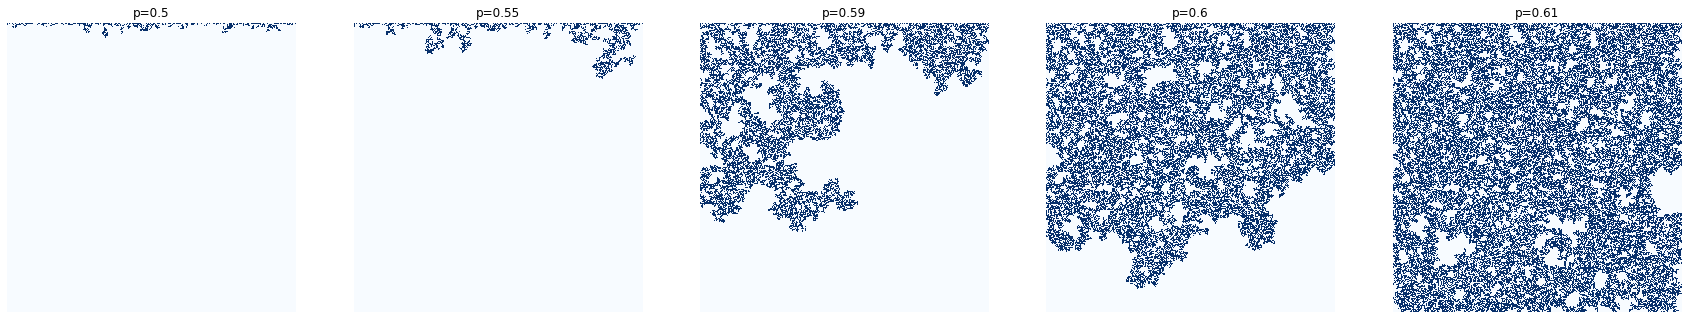
\includegraphics[width=1 \textwidth]{./Pictures/evolution2.png}
    \caption{Évolution de la percolation sur une grille $500\times 500$ en fonction de la probabilité d'ouverture}
    \label{fig:evol}
\end{figure}

Ces simulations mettent en évidence que la probabilité critique pour notre modélisation est autour de $0.6$\ . Attention cependant, dans la partie théorique qui suit, on montrera que la probabilité critique vaut $0.5$, mais le modèle qui y sera étudié est légeremment différent car ce sont les arêtes qui y sont ouvertes ou fermées, et non pas les cases. Ici, dans ce modèle dit de ``percolation par sites'', la valeur critique exacte n'est pas explicitement connue. \\

On peut ensuite calculer expérimentalement le diagramme de phase de notre modèle, c'est à dire la probabilité de percolation en fonction de la probabilité d'ouverture.
\begin{figure}[htbp]
    \centering
    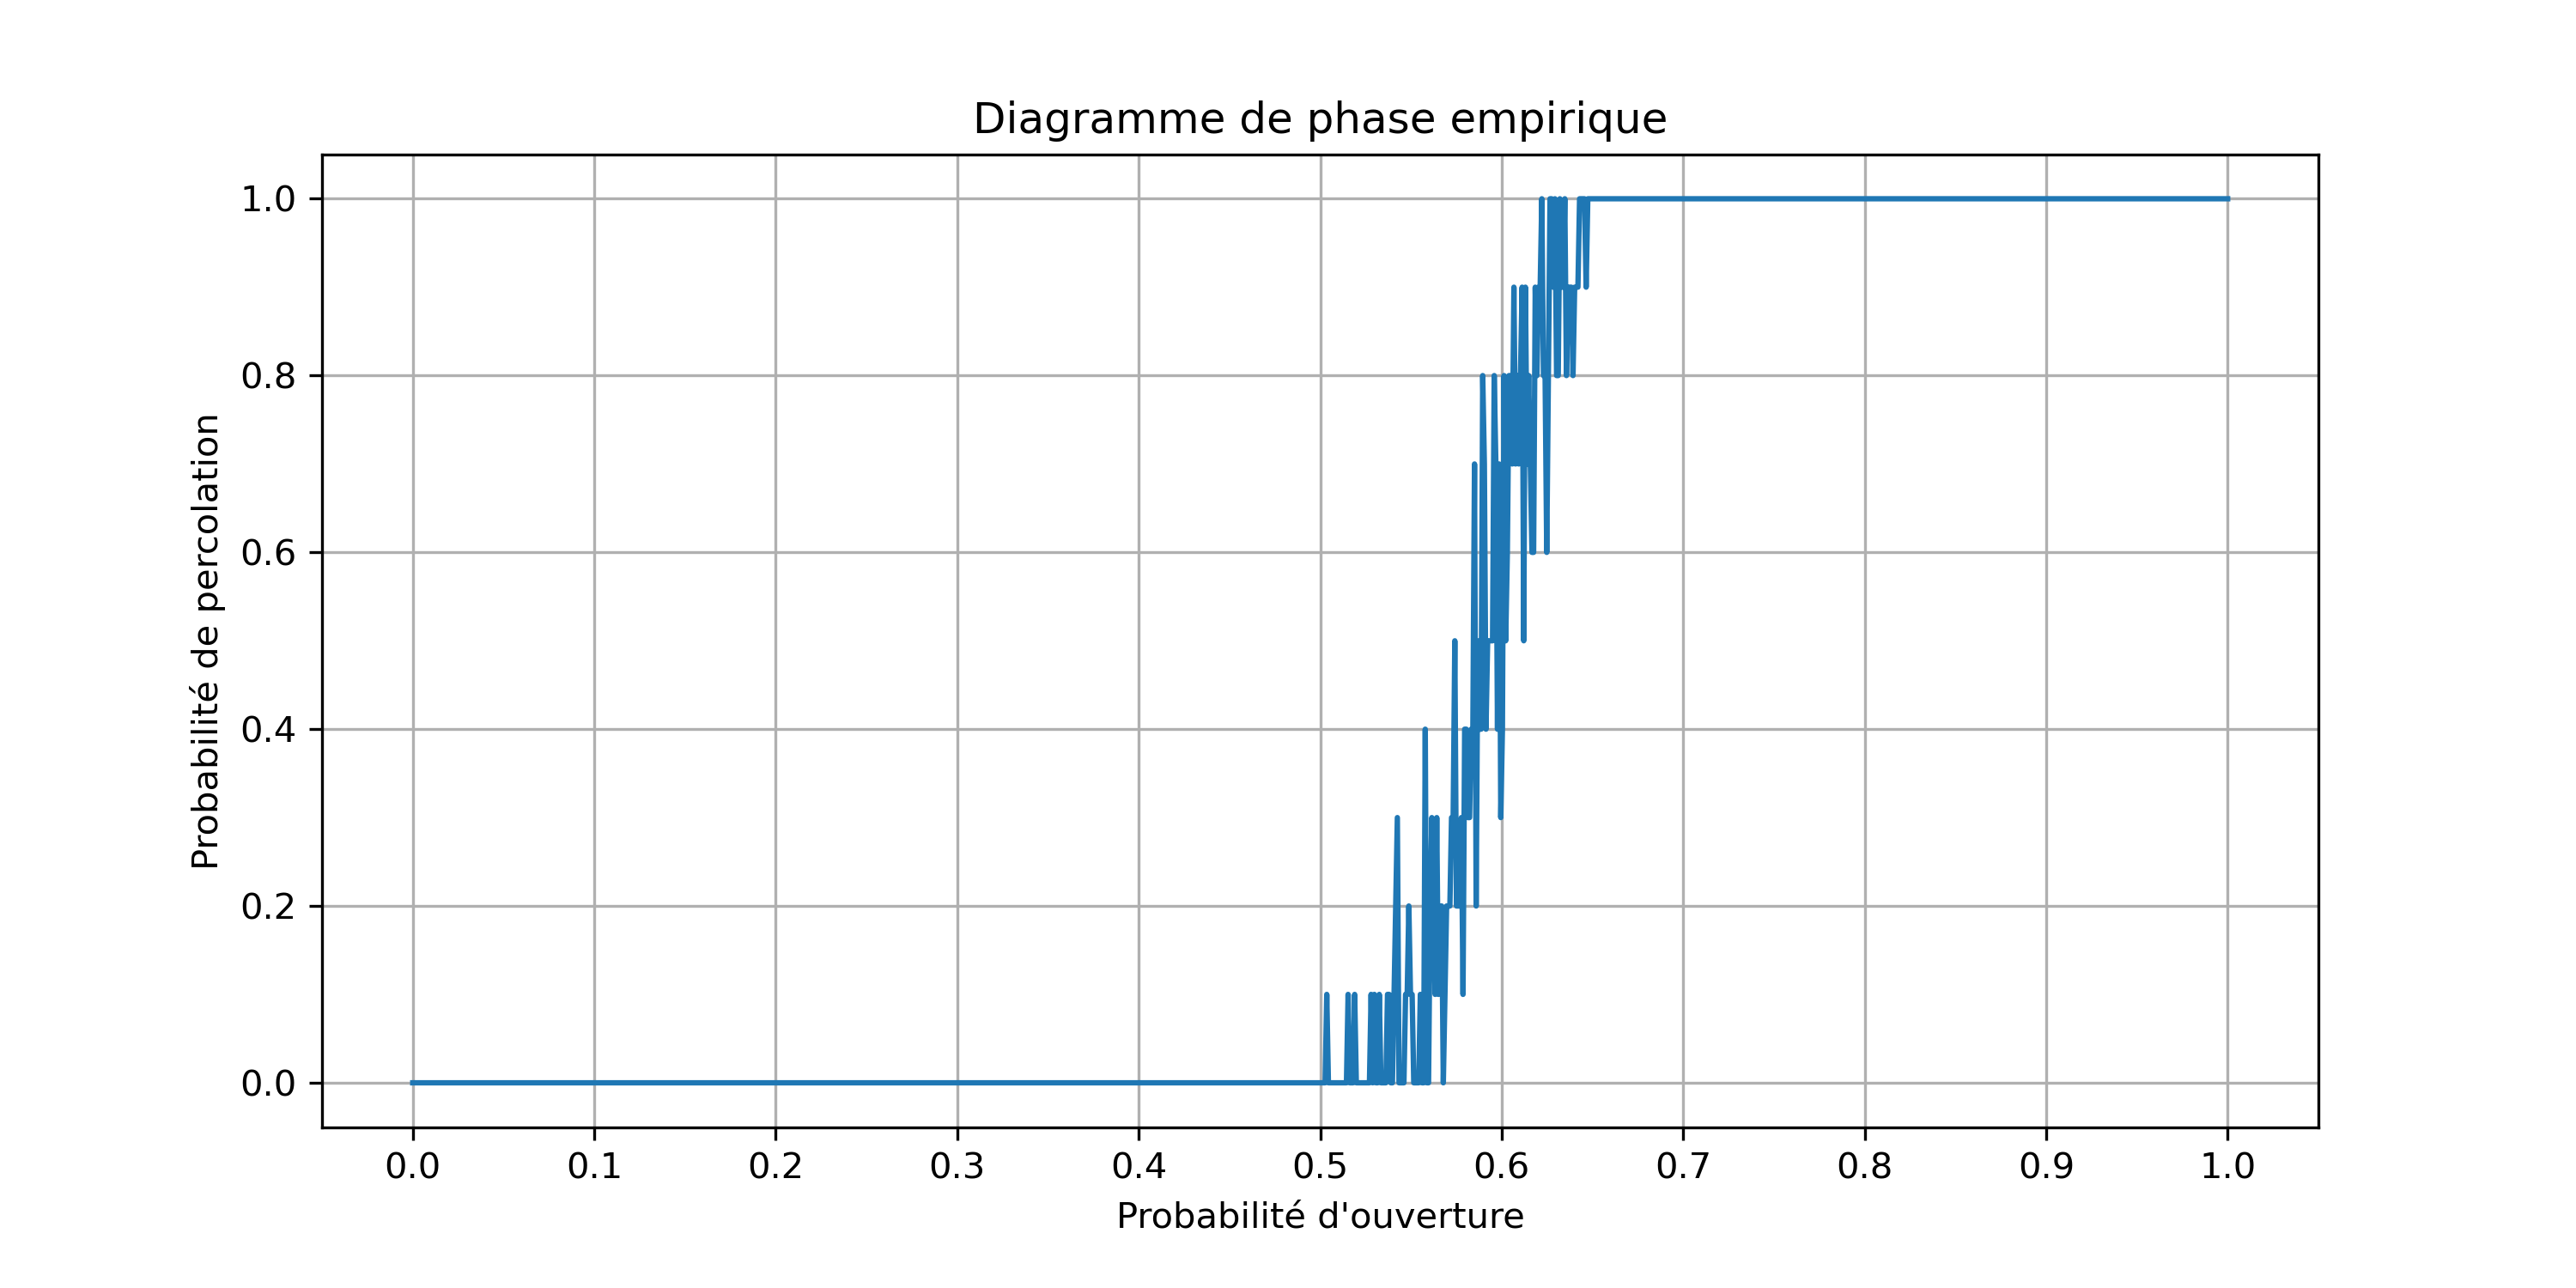
\includegraphics[width=0.6 \textwidth]{./Pictures/percolation_probability.png}
    \caption{Diagramme de phase expérimental pour une grille $100\times 100$}
    \label{fig:evol}
\end{figure}

On peut le comparer au diagramme de phase théorique de la percolation ``classique'' précédemment évoquée, et on constate que dans le modèle par sites, la percolation presque sûre est atteinte bien plus rapidement : 

\begin{figure}[htbp]
    \centering
    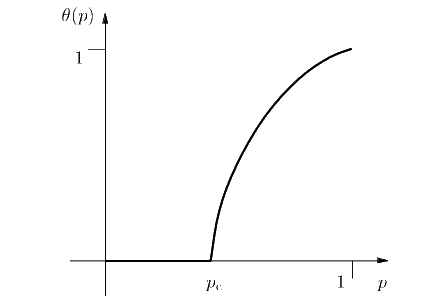
\includegraphics[width=0.4 \textwidth]{./Pictures/ph_th.png}
    \caption{Diagramme de phase théorique dans le cas de percolation standard \cite{grimmett}}
    \label{fig:evol}
\end{figure}

\subsection{Plus grande composante connexe}
\ \ \ \ \ Dans la partie théorique suivante, nous aurons besoin d'un résultat d'unicité de la plus grande composante connexe lorsqu'il y a percolation, c'est à dire unicité de la composante connexe infinie car en théorie la grille est infinie. Au vu de la difficulté de la preuve rigoureuse de ce lemme, on se propose plutôt de le mettre en évidence expérimentalement : les graphes suivants ont leurs composantes connexes coloriés, on observe bien que les composantes qu'il y a unicité de la composante qui atteint le bas de la grille. 

\begin{figure}[htp]

\centering
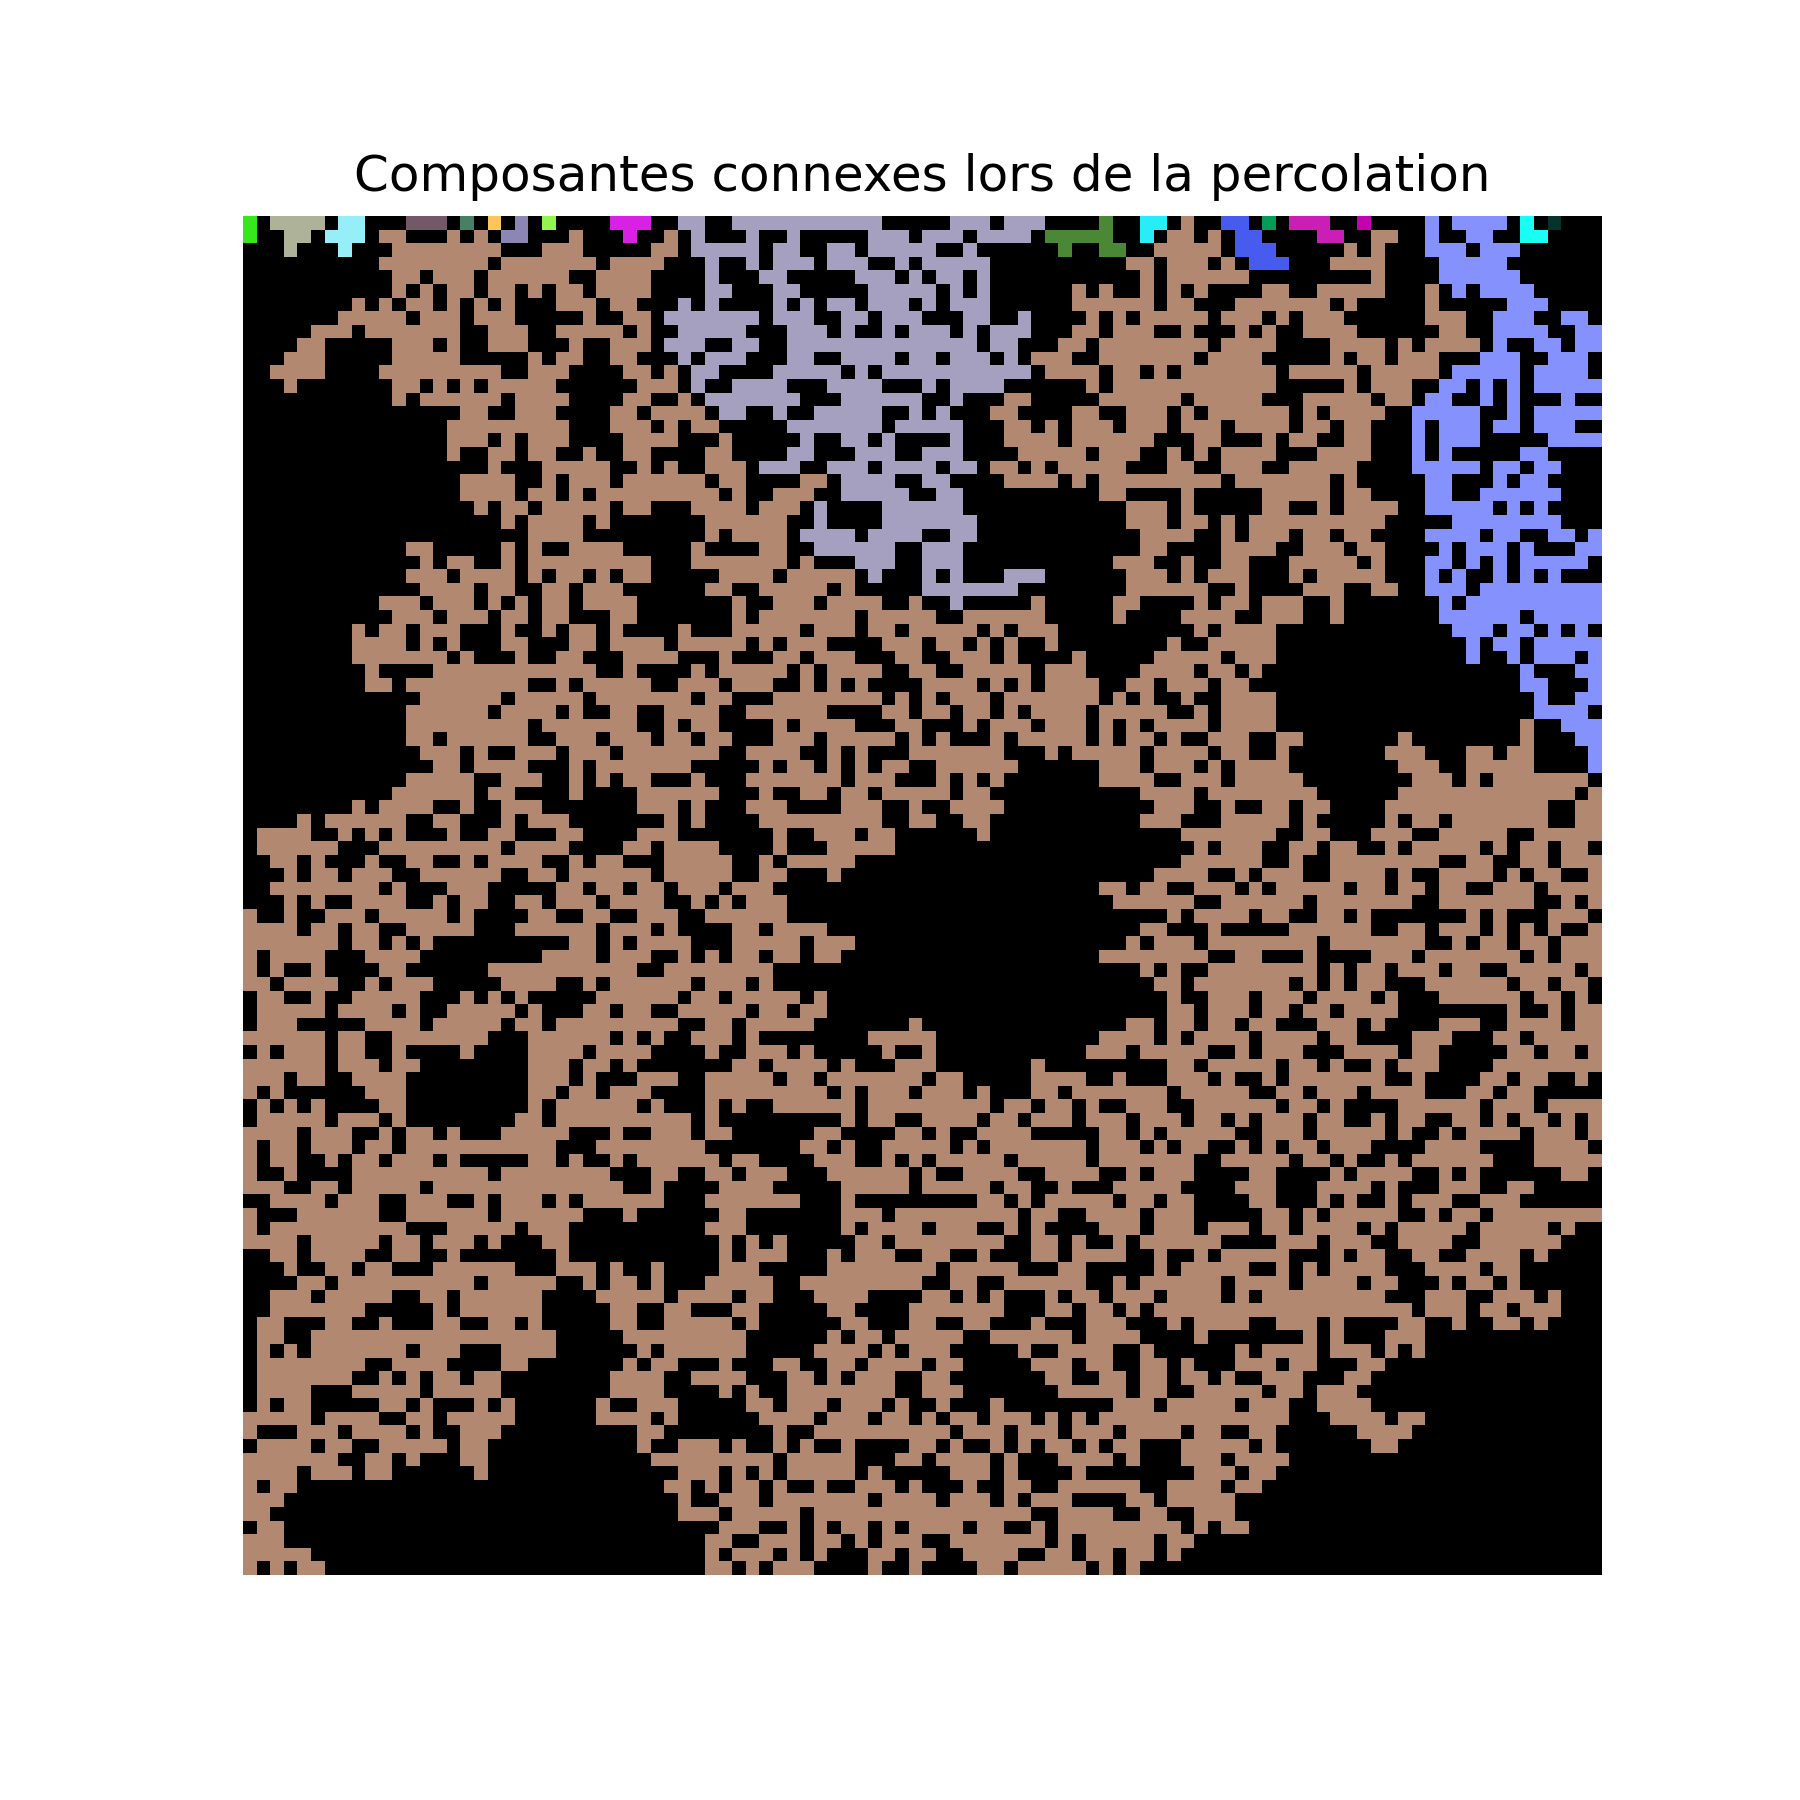
\includegraphics[width=.3333\textwidth]{./Pictures/cc100.png}\hfill
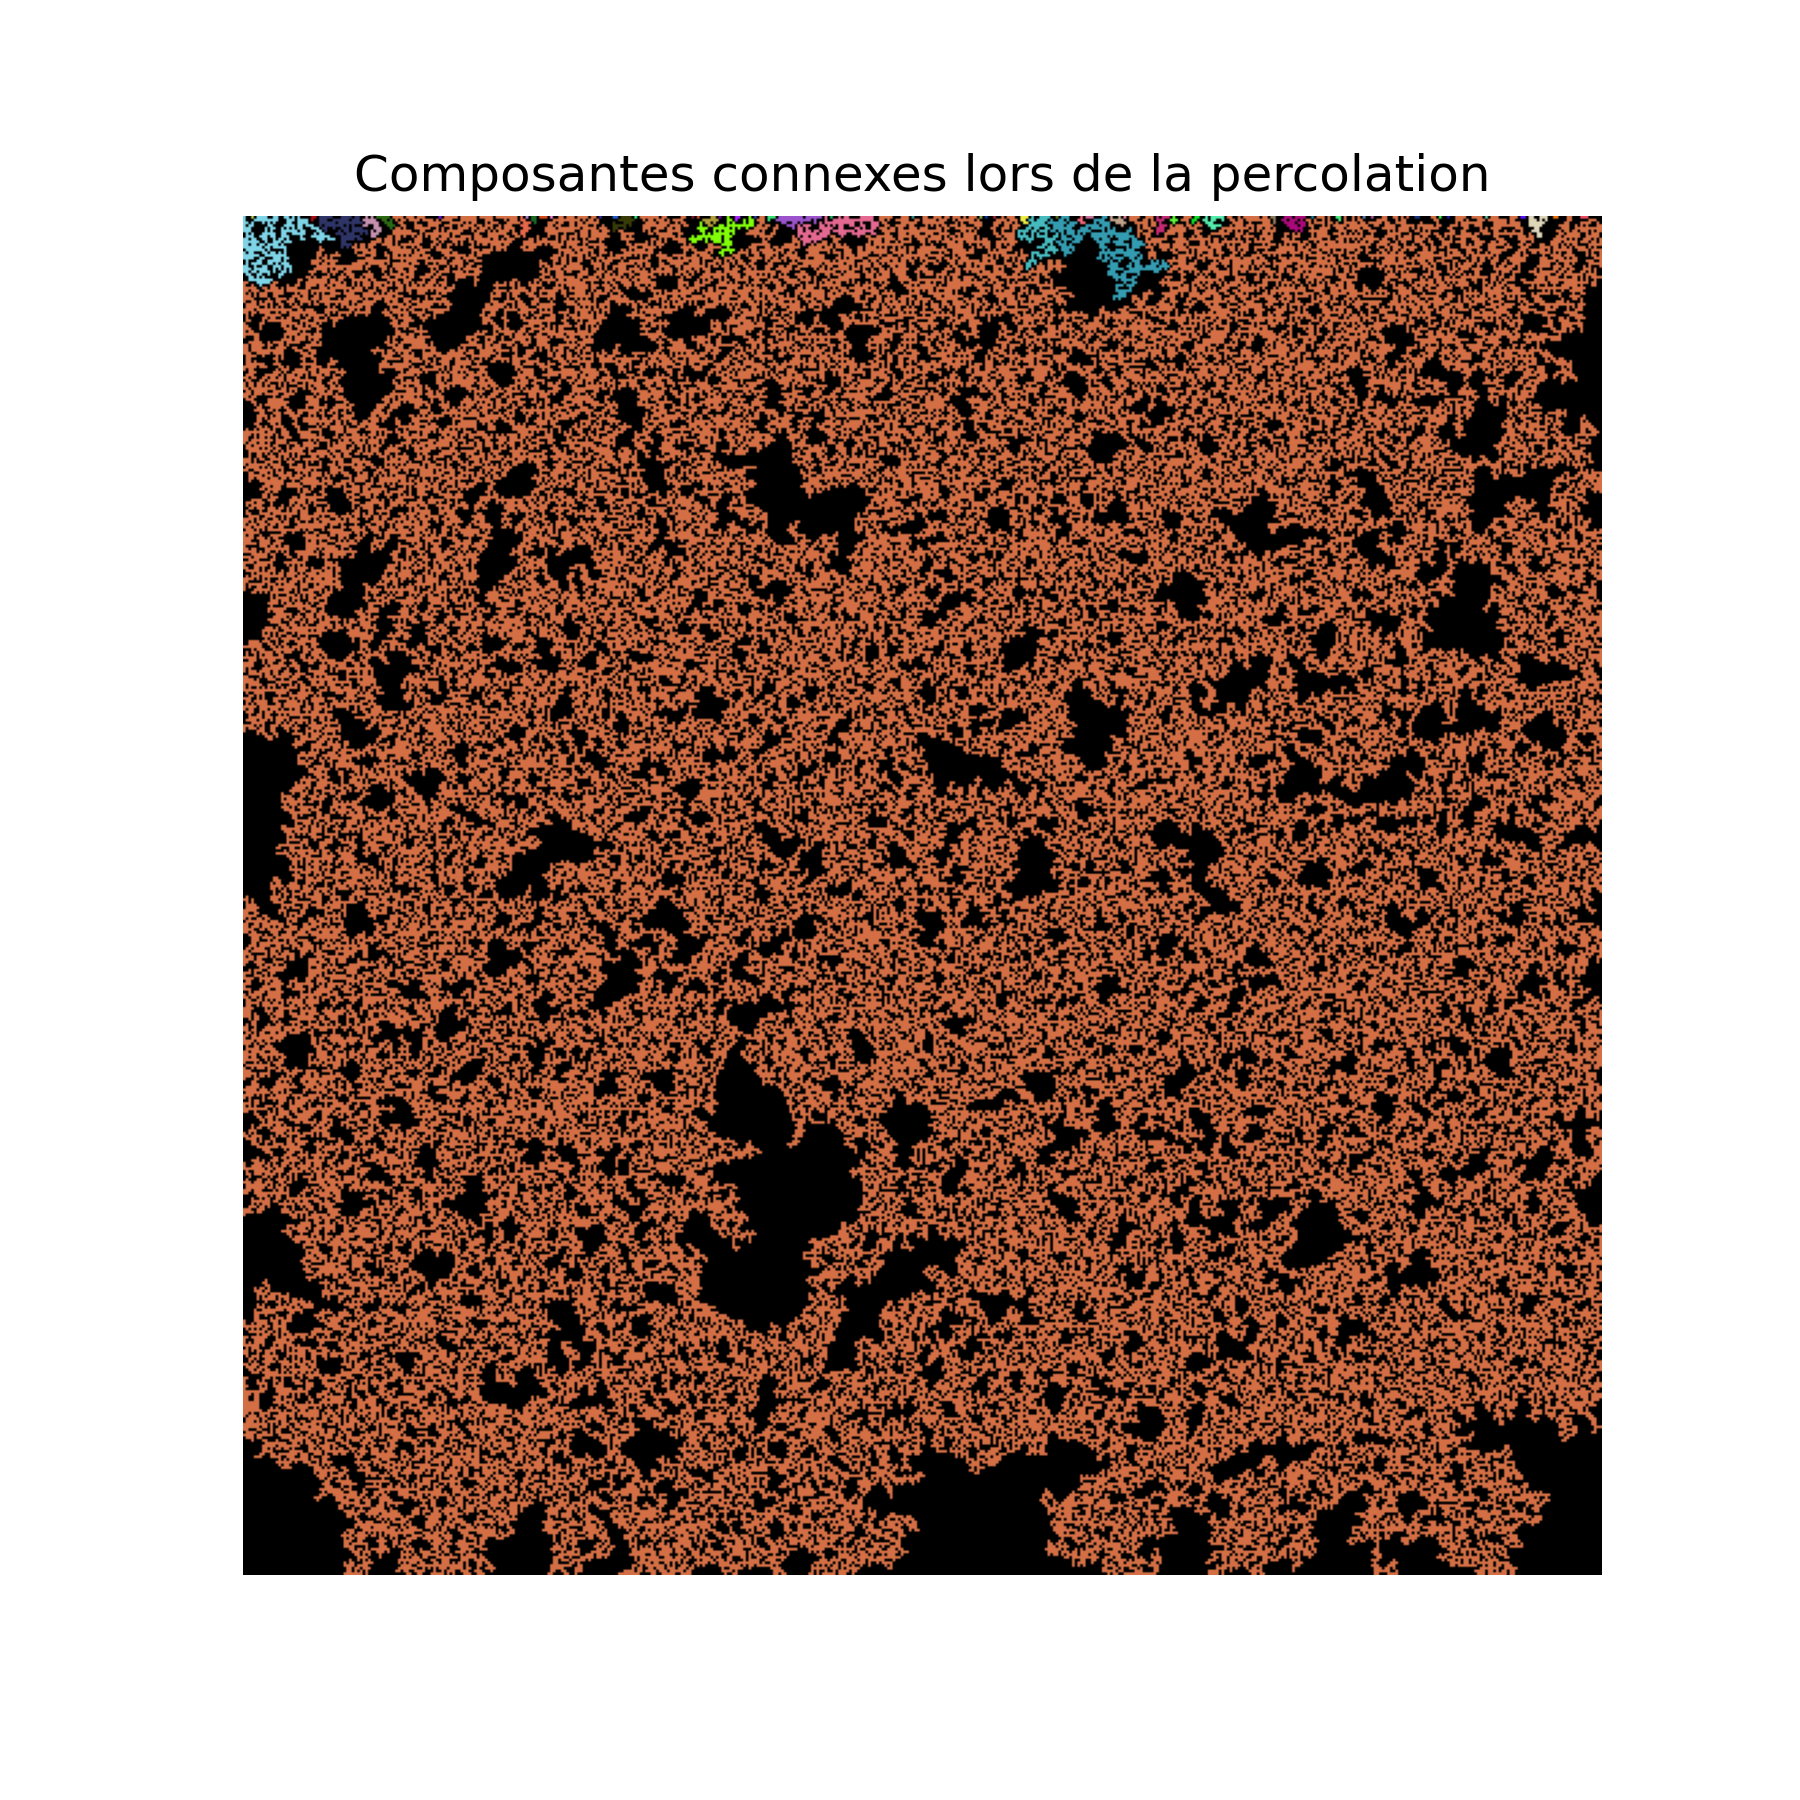
\includegraphics[width=.3333\textwidth]{./Pictures/cc500.png}\hfill
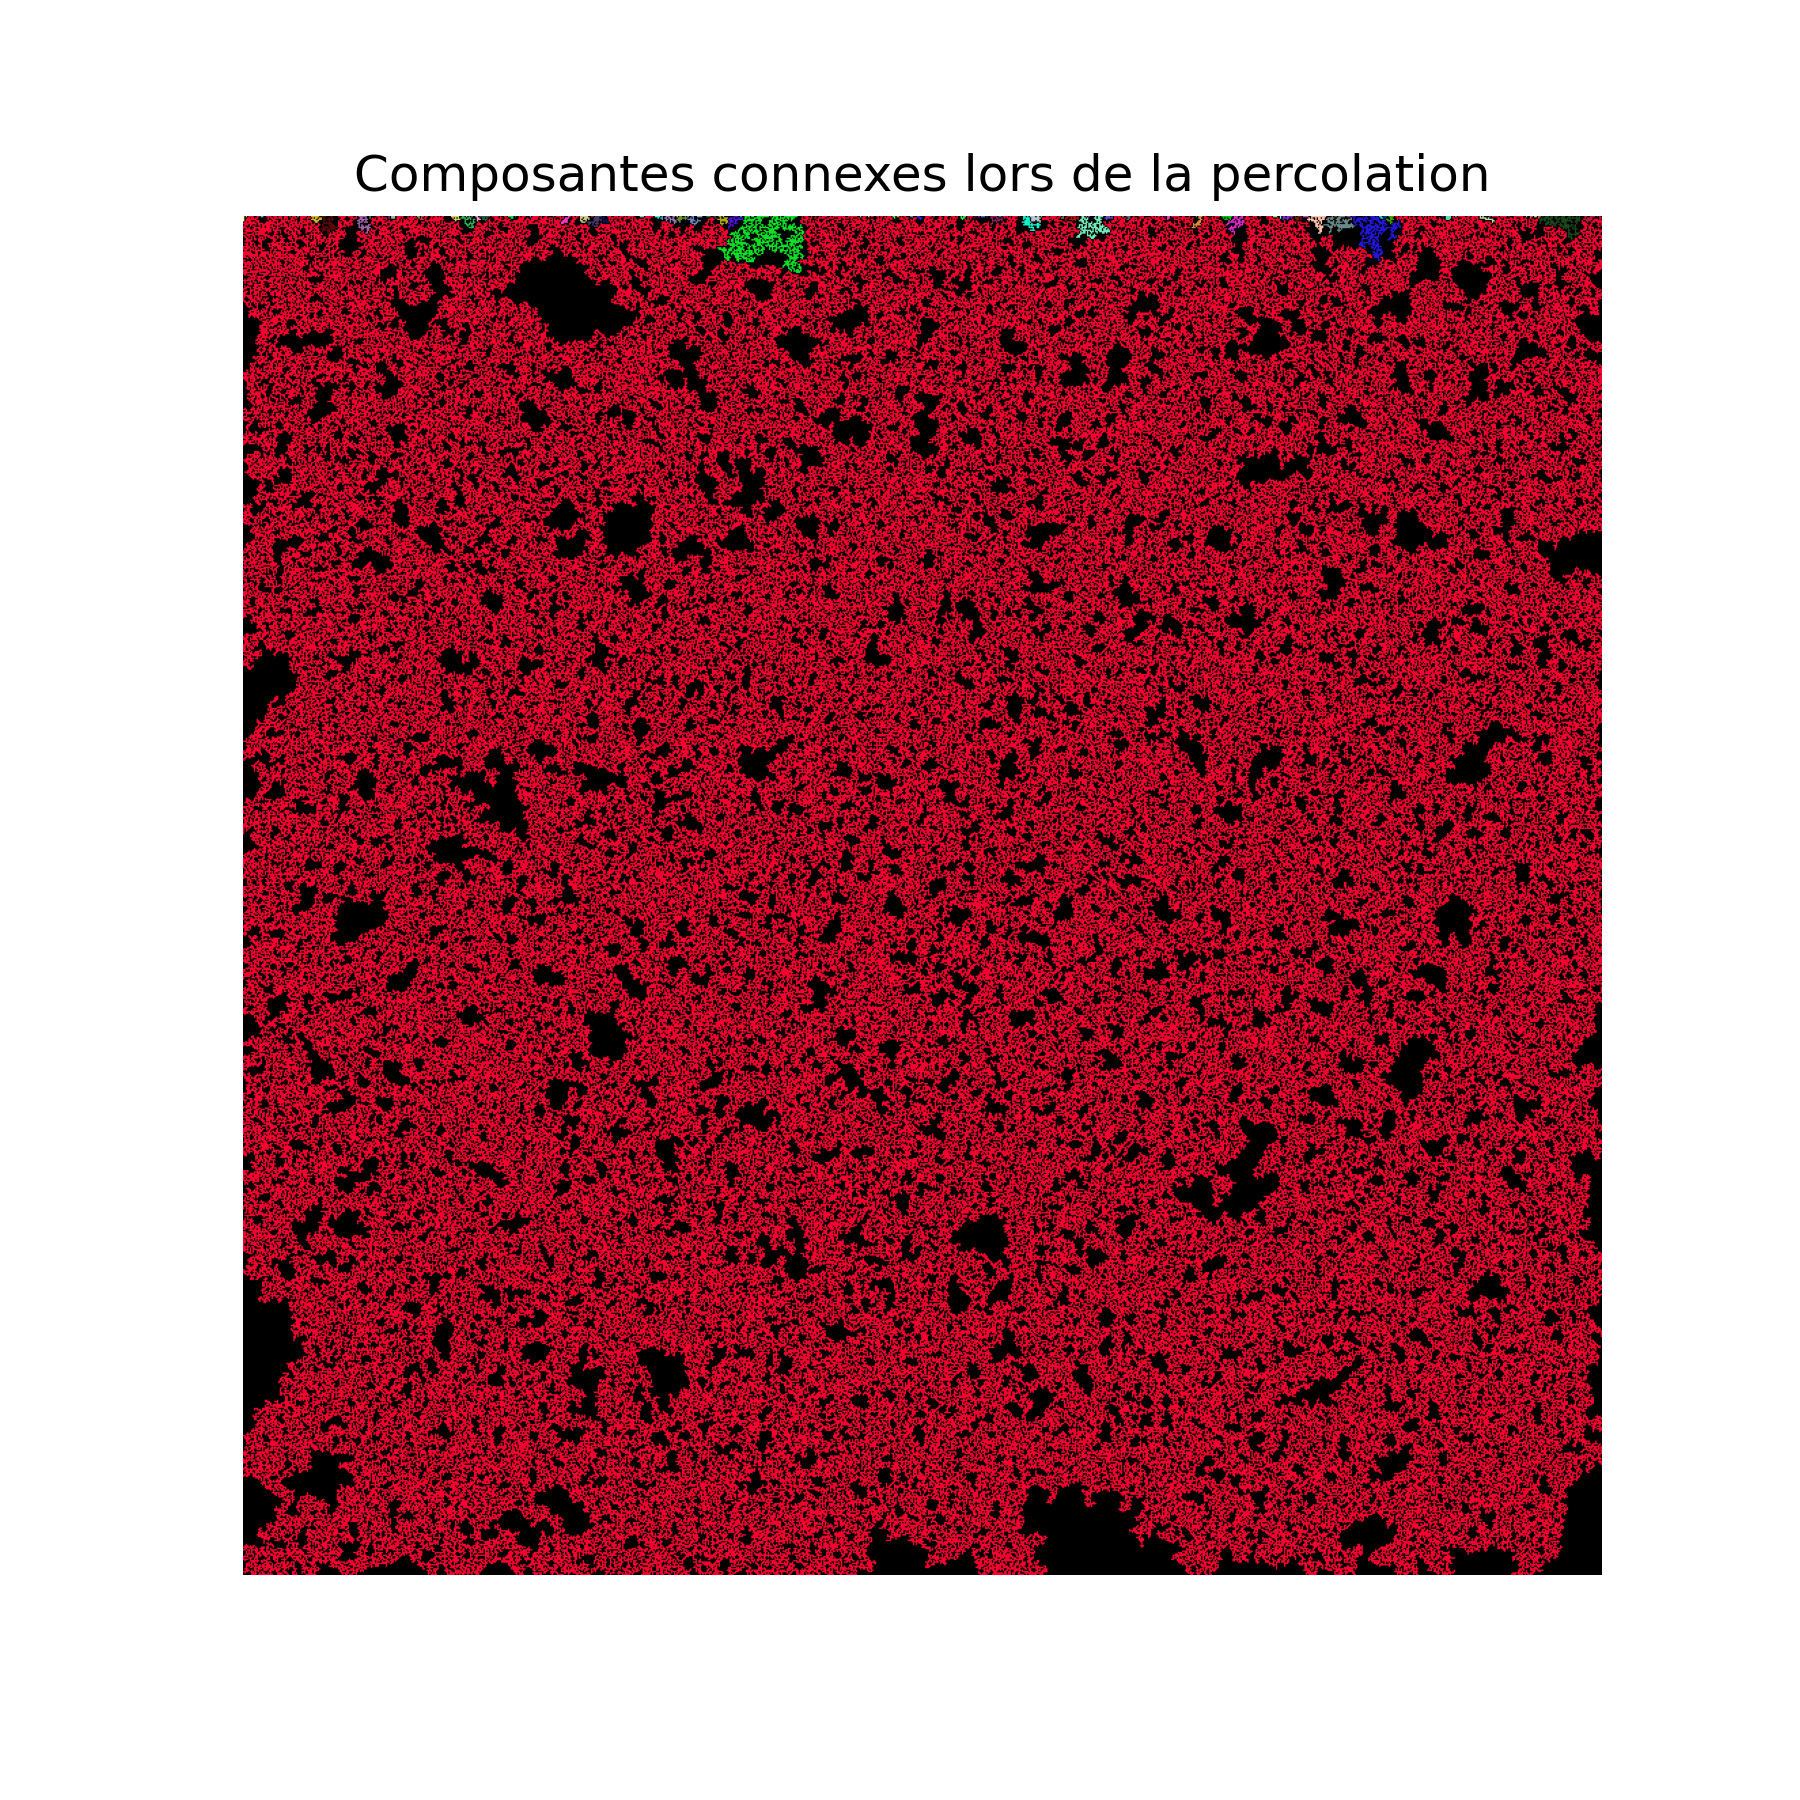
\includegraphics[width=.3333\textwidth]{./Pictures/cc1000.png}

\caption{Composantes connexes coloriées sur des grilles carrées de taille $100$, $500$ et $1000$ à $p=0.6$}
\label{fig:figure3}

\end{figure}

\newpage
\printbibliography[heading=bibintoc, title={Références}]

\end{document}
